% A power-loss-tolerant, supercapacitor-powered logger on the MSP430FR5994
% Build:  pdflatex lab_report ; bibtex lab_report ; pdflatex lab_report ; pdflatex lab_report
\documentclass[conference]{IEEEtran}
\IEEEoverridecommandlockouts

\usepackage[T1]{fontenc}
\usepackage[utf8]{inputenc}
\usepackage{cite}
\usepackage{amsmath,amssymb}
\usepackage{graphicx}
\usepackage{booktabs}
\usepackage{tabularx}
\usepackage{float}
\usepackage{array}
\usepackage{siunitx}
\usepackage{enumitem}
\usepackage{xcolor}
\usepackage{url}
\usepackage{tikz}
\usetikzlibrary{positioning,arrows.meta,fit,calc,backgrounds,shapes.geometric}
\usepackage{pgfplots}
\usepgfplotslibrary{groupplots}
\pgfplotsset{compat=1.18}
\usepackage[hidelinks]{hyperref}

\sisetup{detect-all, per-mode=symbol}
\newcommand{\uA}{\,\si{\micro\ampere}}
\newcommand{\mA}{\,\si{\milli\ampere}}
\newcommand{\uC}{\,\si{\micro\coulomb}}
\newcommand{\code}[1]{\texttt{#1}}
\newcolumntype{L}{>{\raggedright\arraybackslash}X}
\setlist{itemsep=1pt,topsep=3pt}

\begin{document}

\title{A Power-Loss-Tolerant, Supercapacitor-Powered Data Logger on the MSP430FR5994: Driver Design and Energy Characterization%
\thanks{\textbf{AI-assistance disclosure:} this work was carried out with the assistance of Claude (Anthropic), an AI assistant, which wrote the firmware, analysed the measurement data and drafted this paper under the author's direction. All hardware experiments were run by the author.}}

\author{\IEEEauthorblockN{Jo\~{a}o Gabriel Peixoto}
\IEEEauthorblockA{Pontifical Catholic University of Rio de Janeiro (PUC-Rio)\\
Rio de Janeiro, Brazil\\
joaogdrumond@aluno.puc-rio.br}}

\maketitle

\begin{abstract}
Devices powered by small energy stores must keep working through supply collapses without losing their state. This paper presents a three-layer firmware stack for the MSP430FR5994 LaunchPad, powered only by its onboard \SI{0.22}{\farad} supercapacitor, that logs supply voltage and die temperature every \SI{2}{\second}. Every errata item that affects the chosen peripherals is handled in the drivers. State is protected by a two-slot, CRC-checked checkpoint store in FRAM, and the logger drops into LPM3.5 below \SI{2.2}{\volt} and resumes at \SI{2.6}{\volt}. A UART command console gives access to the data without a debugger. The checkpoint store survived 36 abrupt power cuts and a deterministic fault-injection sequence covering every step of a save with no lost or corrupted state. The deep-sleep path woke exactly on the RTC minute nine times out of nine. EnergyTrace measurements reduced the average current from \SI{780}{\micro\ampere} for a first driver demo to 3.2--4.4\uA{} for the final logger, and showed that an idle console costs nothing measurable. An 82-minute run on the supercapacitor alone measured a total drain of 5.4\uA{} from the voltage slope, which includes the capacitor's own leakage. That rate gives about 8.5\,h of logging from the 2.96\,V the charge reached. Two measurement pitfalls are documented: a debugger in control inflated the sleep current to 170\uA, and EnergyTrace's absolute floor shifts by about 1\uA{} between sessions, which motivates comparing firmware variants inside a single capture.
\end{abstract}

\begin{IEEEkeywords}
intermittent computing, energy harvesting, FRAM, checkpointing, MSP430, low-power firmware, energy measurement
\end{IEEEkeywords}

% =====================================================================
\section{Introduction}

Batteryless and energy-harvesting sensors run from small stores such as capacitors, and their supply can collapse at any moment~\cite{hester2017future,lucia2017snapl}. Firmware for such devices must preserve its state across power losses, avoid spending energy it does not have, and recover by itself. Microcontrollers with ferroelectric RAM (FRAM) make the first goal practical: FRAM is non-volatile, byte-addressable and writable at low energy, so program state can be saved often~\cite{jayakumar2014quickrecall}.

This work builds such a system from the register level on the MSP-EXP430FR5994 LaunchPad~\cite{ti_slau678}, using its onboard \SI{0.22}{\farad} supercapacitor as the only energy source. The application is a logger that samples its own supply voltage and die temperature every \SI{2}{\second}. The main contributions are:
\begin{itemize}
  \item a layered driver stack (core, sensing and persistence, communication) that applies every relevant item of the device errata~\cite{ti_slaz681};
  \item a power-loss-safe checkpoint store with an explicit commit point, validated by random power cuts and by deterministic fault injection at each step of a save;
  \item a supply-aware power policy that moves between LPM3 logging and LPM3.5 deep sleep with continuous timekeeping;
  \item an energy characterization with EnergyTrace, including a method for comparing firmware variants within a single capture, which the measurements showed to be necessary.
\end{itemize}

Section~\ref{sec:related} reviews related work, Section~\ref{sec:design} describes the design, Section~\ref{sec:method} the measurement method, Section~\ref{sec:results} the results, and Section~\ref{sec:discussion} the lessons and limitations. Section~\ref{sec:conclusion} concludes and lists future work. A detailed experiment record follows the references.

% =====================================================================
\section{Background and Related Work}
\label{sec:related}

\emph{Intermittent computing} studies programs that run across frequent power failures~\cite{lucia2017snapl}. Mementos~\cite{ransford2011mementos} inserts trigger points at compile time and checkpoints volatile state to flash when the supply voltage is low. Hibernus~\cite{balsamo2015hibernus} instead watches the supply and takes a single snapshot to non-volatile memory as late as possible, when failure is imminent. QuickRecall~\cite{jayakumar2014quickrecall} uses FRAM as unified memory on an MSP430FR5739, so that only registers need saving, which makes checkpoints cheap. DINO~\cite{lucia2015dino} points out that checkpointing volatile state alone can leave non-volatile data inconsistent after re-execution, and proposes task boundaries with data versioning. Capybara~\cite{colin2018capybara} addresses the energy store itself, reconfiguring storage capacity to match the energy each task needs.

This work sits at the application level of that design space. The state that matters (counters and a sample log) is small and explicit, so it is saved as a whole after every change, and its consistency is guaranteed by an atomic two-copy commit in the spirit of shadow paging~\cite{lorie1977physical}, with a CRC~\cite{koopman2004crc} to detect torn or corrupted copies. Like Hibernus, the system reacts to its supply voltage, but it reacts by entering the device's LPMx.5 shutdown mode~\cite{ti_slau367} and waiting for recovery, instead of preserving an execution context. The focus is the complete embedded system: drivers, errata, power policy and measured energy.

% =====================================================================
\section{System Design}
\label{sec:design}

\subsection{Platform}

The MSP430FR5994 has 256\,KB of FRAM, 8\,KB of SRAM, a 12-bit ADC with an internal reference and temperature sensor, a calendar RTC and four eUSCI\_A UARTs~\cite{ti_slase54}. On the LaunchPad, the supercapacitor ties directly to the 3.3\,V rail when jumper J8 is in its ``use'' position, so the supply voltage VCC is the supercapacitor voltage~\cite{ti_slau678}. The onboard eZ-FET debugger provides programming, a USB backchannel UART on eUSCI\_A0, and EnergyTrace energy measurement~\cite{ti_slaa603}.

\begin{figure*}[t]
\centering
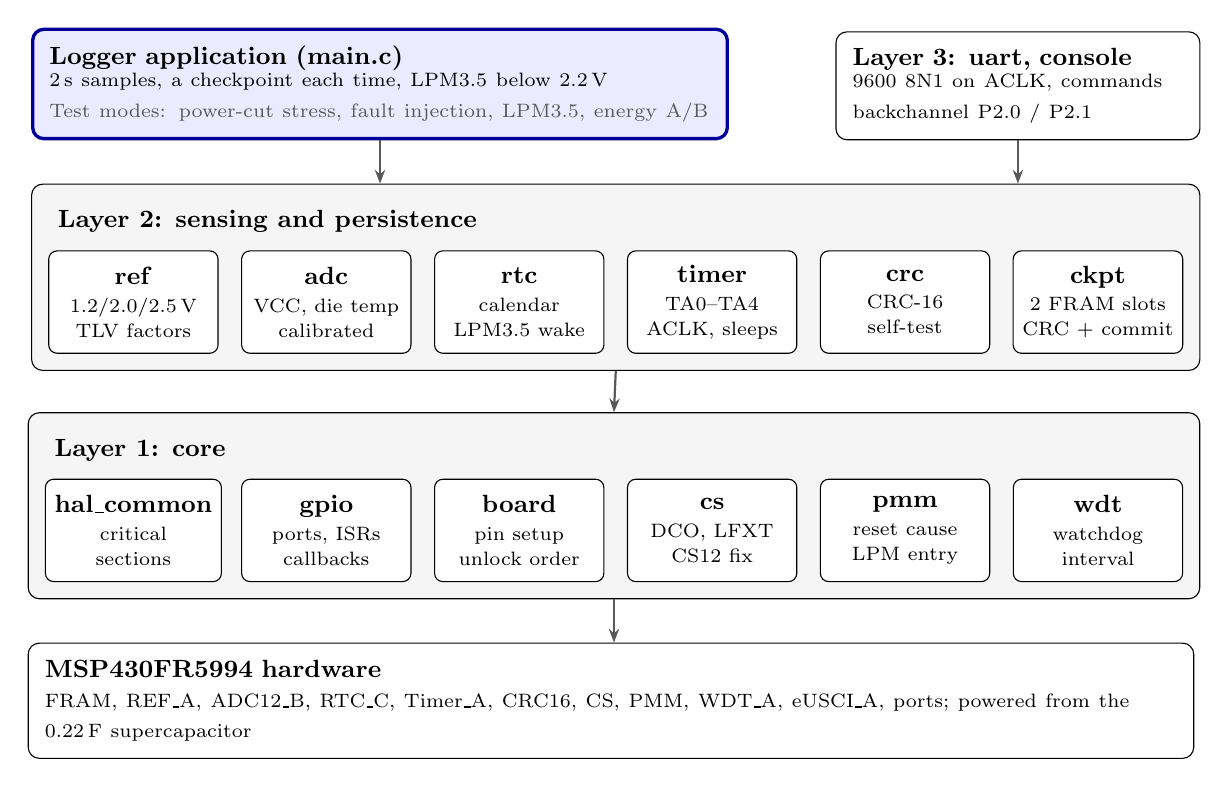
\begin{tikzpicture}[
  font=\small,
  drv/.style={draw, rounded corners=3pt, minimum width=2.15cm, minimum height=1.3cm, align=center, fill=white},
  lay/.style={draw, rounded corners=4pt, fill=gray!8, inner sep=6pt},
  arr/.style={-{Stealth[length=5pt]}, thick, gray!70!black}
]
  \node[drv] (ref)   at (0,0)     {\textbf{ref}\\[-1pt]\scriptsize 1.2/2.0/2.5\,V\\[-2pt]\scriptsize TLV factors};
  \node[drv] (adc)   at (2.45,0)  {\textbf{adc}\\[-1pt]\scriptsize VCC, die temp\\[-2pt]\scriptsize calibrated};
  \node[drv] (rtc)   at (4.9,0)   {\textbf{rtc}\\[-1pt]\scriptsize calendar\\[-2pt]\scriptsize LPM3.5 wake};
  \node[drv] (tim)   at (7.35,0)  {\textbf{timer}\\[-1pt]\scriptsize TA0--TA4\\[-2pt]\scriptsize ACLK, sleeps};
  \node[drv] (crc)   at (9.8,0)   {\textbf{crc}\\[-1pt]\scriptsize CRC-16\\[-2pt]\scriptsize self-test};
  \node[drv] (ckpt)  at (12.25,0) {\textbf{ckpt}\\[-1pt]\scriptsize 2 FRAM slots\\[-2pt]\scriptsize CRC + commit};
  \node[anchor=south west] (l2t) at ($(ref.north west)+(0,0.1)$) {\textbf{Layer 2: sensing and persistence}};
  \node[drv] (hal)   at (0,-2.9)     {\textbf{hal\_common}\\[-1pt]\scriptsize critical\\[-2pt]\scriptsize sections};
  \node[drv] (gpio)  at (2.45,-2.9)  {\textbf{gpio}\\[-1pt]\scriptsize ports, ISRs\\[-2pt]\scriptsize callbacks};
  \node[drv] (board) at (4.9,-2.9)   {\textbf{board}\\[-1pt]\scriptsize pin setup\\[-2pt]\scriptsize unlock order};
  \node[drv] (cs)    at (7.35,-2.9)  {\textbf{cs}\\[-1pt]\scriptsize DCO, LFXT\\[-2pt]\scriptsize CS12 fix};
  \node[drv] (pmm)   at (9.8,-2.9)   {\textbf{pmm}\\[-1pt]\scriptsize reset cause\\[-2pt]\scriptsize LPM entry};
  \node[drv] (wdt)   at (12.25,-2.9) {\textbf{wdt}\\[-1pt]\scriptsize watchdog\\[-2pt]\scriptsize interval};
  \node[anchor=south west] (l1t) at ($(hal.north west)+(0,0.1)$) {\textbf{Layer 1: core}};
  \begin{scope}[on background layer]
    \node[lay, fit=(ref)(ckpt)(l2t)] (L2) {};
    \node[lay, fit=(hal)(wdt)(l1t)] (L1) {};
  \end{scope}
  \node[draw=blue!60!black, very thick, fill=blue!8, rounded corners=4pt, align=left, text width=8.4cm, inner sep=6pt,
        anchor=south west] (app) at ($(L2.north west)+(0,0.55)$)
        {\textbf{Logger application (main.c)}\\ \scriptsize 2\,s samples, a checkpoint each time, LPM3.5 below 2.2\,V\\ \scriptsize\color{gray!70!black} Test modes: power-cut stress, fault injection, LPM3.5, energy A/B};
  \node[draw, rounded corners=4pt, align=left, text width=4.2cm, inner sep=6pt, anchor=south east, fill=white]
        (l3) at ($(L2.north east)+(0,0.55)$)
        {\textbf{Layer 3: uart, console}\\ \scriptsize 9600 8N1 on ACLK, commands\\ \scriptsize backchannel P2.0 / P2.1};
  \node[draw, rounded corners=4pt, align=left, anchor=north west, inner sep=6pt, text width=14.38cm]
        (hw) at ($(L1.south west)+(0,-0.55)$)
        {\textbf{MSP430FR5994 hardware}\\ \scriptsize FRAM, REF\_A, ADC12\_B, RTC\_C, Timer\_A, CRC16, CS, PMM, WDT\_A, eUSCI\_A, ports; powered from the 0.22\,F supercapacitor};
  \draw[arr] (app.south) -- (app.south |- L2.north);
  \draw[arr] (l3.south) -- (l3.south |- L2.north);
  \draw[arr] (L2.south) -- (L1.north);
  \draw[arr] (L1.south) -- (L1.south |- hw.north);
\end{tikzpicture}
\caption{Firmware architecture. The application uses drivers from all layers and never touches peripheral registers directly, so every test mode runs on the same drivers as the logger.}
\label{fig:arch}
\end{figure*}

\subsection{Driver layers}

Fig.~\ref{fig:arch} shows the three layers.
\emph{Layer~1} brings up the board in the order the hardware requires: it holds the watchdog, latches the reset cause, puts every pin into a low-power state, configures the crystal pins, and only then releases the I/O lock (LOCKLPM5). Port interrupt flags are cleared only after a cold start, because after an LPMx.5 wake they hold the wake event~\cite{ti_slau367}. The clock driver runs the DCO at 8\,MHz and starts the 32.768\,kHz crystal (LFXT) with a timeout and a fall-back to the internal VLO.
\emph{Layer~2} adds the voltage reference, ADC (VCC through the internal \(\tfrac{1}{2}\)\,AVCC divider, die temperature through the calibrated sensor), RTC, timers, CRC, and the checkpoint store.
\emph{Layer~3} adds an interrupt-driven UART driver and a line-based command console.

Table~\ref{tab:errata} lists the errata and datasheet constraints the drivers handle. The most consequential are PMM31/PMM32: entering LPM2--4 with FRAM powered can fail, so every low-power entry runs from RAM and powers FRAM down first~\cite{ti_slaz681}.

\begin{table}[t]
\caption{Errata and constraints handled in the drivers~\cite{ti_slaz681,ti_slase54}}
\label{tab:errata}
\centering\footnotesize
\begin{tabularx}{\columnwidth}{@{}lL@{}}
\toprule
Item & Handling \\
\midrule
PMM31/32 & LPM2--4 entry from RAM with FRAM powered down; ADC used in active mode only \\
CS12 & Clock dividers $\geq$\,/4 around a DCO change, $\sim$10\,\textmu s settle \\
ADC42 & BUSY checked before every conversion \\
ADC71 & ENC and SC set in separate writes \\
ADC67 & API to override the TLV temperature calibration \\
USCI42 & UART end of transmission from UCBUSY, not UCTXCPTIFG \\
FRAM & One wait state above 8\,MHz (NWAITS) \\
REF/AVCC & 1.2\,V reference below 2.4\,V VCC; each reference needs its minimum AVCC \\
LPMx.5 & RTC and ports reconfigured before LOCKLPM5 is cleared; wake flags kept \\
\bottomrule
\end{tabularx}
\end{table}

\subsection{Power-loss-safe checkpoint store}

The application state (boot, power-loss and deep-sleep counters, sample count, minimum VCC, and a 16-entry log of time, VCC and temperature) lives in RAM and is saved to FRAM after every change. The store keeps two slots in persistent FRAM. Each holds a magic word, length, sequence number, CRC-16/CCITT and payload. A save always writes the slot that does \emph{not} hold the newest valid copy, in this order:
\begin{enumerate}
  \item mark the slot invalid;
  \item write payload, length and sequence number;
  \item write the CRC over length, sequence and payload;
  \item mark the slot valid (the commit point).
\end{enumerate}
Restore returns the valid slot with the highest sequence number. A power cut before step~4 leaves the previous copy as the newest valid one. A cut after it leaves the new copy. A torn or bit-flipped slot fails its CRC and is ignored. The CRC is computed by the hardware CRC16 module and checked at boot against a software reference.

\subsection{Long history and clock recovery}

The checkpoint payload holds only the newest 16 samples (32\,s). For discharge experiments, a separate ring of 1600 records (22.4\,KB of FRAM) stores one record every 60 samples (2\,min) while logging, plus one at each boot, deep-sleep entry, minute wake and resume. That covers about 21\,h of logging followed by 8\,h of minute wakes. Each record is committed like a checkpoint slot: it is invalidated first and its one-byte valid mark is written last. A 16-bit sequence number orders the records, and a persistent hint lets a boot find the newest record without scanning the ring. The hint is verified, and repaired if a cut left it one record behind.

A brown-out resets the RTC to its default date. The RTC driver keeps the time whenever the RTC is still running with a valid date, which covers LPMx.5 wakes and resets that do not clear it. After a real power loss, the firmware restarts the clock one second after the newest logged time, so timestamps never run backwards. The restored clock is then behind by the length of the outage, and the boot record flags it as restored.

\subsection{Supply-aware power policy}

Fig.~\ref{fig:fsm} shows the policy. While VCC is at least 2.2\,V, the RTC wakes the CPU from LPM3 every 2\,s to take a sample, save a checkpoint and service a 16\,s watchdog. A green LED flashes for 2\,ms only when a sample lands in log slot~0, i.e.\ once per pass through the 16-entry log. Below 2.2\,V the logger saves, shuts the console down and enters LPM3.5, where only the RTC runs on the crystal~\cite{ti_slau367}. An RTC minute event wakes it. This wake is a reset, so it passes through boot and restore, measures VCC, and returns to LPM3.5 unless VCC has recovered to 2.6\,V. The 400\,mV hysteresis keeps the logger from oscillating at the threshold. A real power loss ends in a brown-out reset and the same restore path. The reference for the VCC measurement is chosen so that it never exceeds what the falling supply can support.

\begin{figure}[t]
\centering
\resizebox{\columnwidth}{!}{%
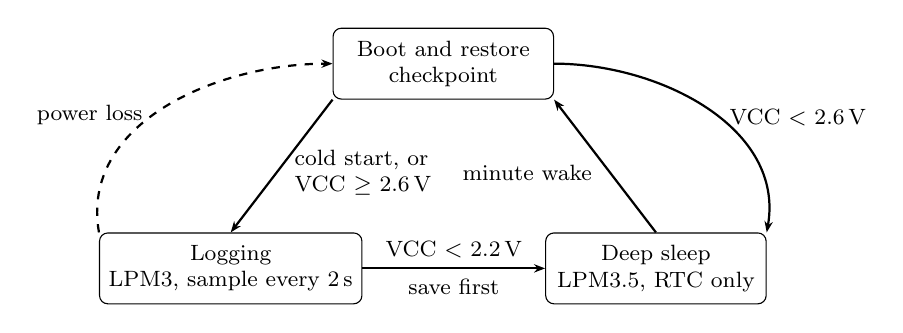
\begin{tikzpicture}[font=\footnotesize,
  st/.style={draw, rounded corners=3pt, align=center, minimum height=9mm, minimum width=2.8cm, fill=white},
  arr/.style={-{Stealth[length=4pt]}, thick}]
  \node[st] (boot) at (0,0)      {Boot and restore\\checkpoint};
  \node[st] (log)  at (-2.7,-2.6) {Logging\\LPM3, sample every 2\,s};
  \node[st] (deep) at (2.7,-2.6)  {Deep sleep\\LPM3.5, RTC only};
  \draw[arr] (boot.south west) -- node[right, pos=0.55, xshift=1mm, align=left] {cold start, or\\VCC $\geq$ 2.6\,V} (log.north);
  \draw[arr] (deep.north) -- node[left, pos=0.45, xshift=-1mm] {minute wake} (boot.south east);
  \draw[arr] (log.east) -- node[above] {VCC $<$ 2.2\,V} node[below] {save first} (deep.west);
  \draw[arr] (boot.east) to[out=0, in=80] node[right, pos=0.55] {VCC $<$ 2.6\,V} (deep.north east);
  \draw[arr, dashed] (log.north west) to[out=100, in=180] node[left, pos=0.45] {power loss} (boot.west);
\end{tikzpicture}}
\caption{Supply-aware power policy with 400\,mV hysteresis. Cold starts, power losses (brown-out resets) and minute wakes from LPM3.5 all pass through checkpoint restore. A wake resumes logging only at VCC $\geq$ 2.6\,V; after a cold start the first sample sends the logger back to deep sleep if VCC is below 2.2\,V.}
\label{fig:fsm}
\end{figure}

\subsection{Command console}

The console runs on the backchannel UART at 9600\,baud, clocked from ACLK (the 32\,kHz crystal). With $N = 32768/9600 = 3.41$, the divider is UCBRx\,=\,3 with modulation pattern UCBRSx\,=\,0x92, from the procedure and table in the user's guide~\cite{ti_slau367}. ACLK keeps running in LPM3, so the CPU sleeps while bytes are sent and received, waking for one short interrupt per byte. The driver computes these settings for any clock and falls back to SMCLK if the crystal has failed, because the VLO is too slow for 9600\,baud. One driver subtlety: reading the interrupt vector register clears the transmit flag. A transmitter that went idle therefore needs that flag set again by software before its interrupt is re-enabled.

The console offers seven commands. \code{help} lists them. \code{status} shows the time and its source, boot reason, counters, VCC and temperature. \code{log} dumps the 16-sample log as CSV, and \code{hist} the long history. \code{time} shows or sets the RTC. \code{stream} prints each sample as it is taken. \code{erase} clears the state. Timestamps are seconds since 2026-01-01, computed from the full calendar date with Hinnant's civil-date algorithms~\cite{hinnant_date}. The implementation was checked against a reference calendar for 49\,000 consecutive days.

% =====================================================================
\section{Measurement Method}
\label{sec:method}

Robustness was tested with three dedicated build modes that store their results in persistent FRAM, so they survive the resets they provoke; results were read with the debugger attached as ``symbols only'', without reflashing. Energy was measured with EnergyTrace on the eZ-FET~\cite{ti_slaa603}, with the supercapacitor jumper J8 removed so that its charging and leakage stay out of the measurement. The CSV export records cumulative energy in 0.1\,\textmu J steps at about 1\,kHz. Currents were derived from energy differences over 20--100\,ms bins, and averages over complete 2\,s sample periods.

Two practices turned out to be essential (Section~\ref{sec:discussion}). Captures must run in EnergyTrace's \emph{Free Run} mode, not under debugger control. Firmware variants are compared \emph{within one capture}: a build switch changes the behaviour after a fixed number of samples, so both variants share the same calibration.

% =====================================================================
\section{Results}
\label{sec:results}

\subsection{Robustness}

Table~\ref{tab:robust} summarizes the robustness experiments (details in Appendix~B).
In the stress test (E3), the firmware saved checkpoints in a tight loop while USB power was unplugged at random. Every field of each saved copy was derived from one counter, so any mixture of old and new data would be detected. After 36 cuts, no restore failed, no copy was inconsistent, and no completed save was lost.
Because unplugging cannot choose where a cut lands, E4 injected a software brown-out reset at each of six points inside a save, then corrupted FRAM directly. In all nine steps the store returned exactly the copy the design predicts: the old copy for cuts before the commit, the new one after it, a fall-back to the older copy for a corrupted newest slot, and an explicit failure when both slots were corrupted.
In E5, the deep-sleep path ran three episodes on USB power, with the low threshold forced by a test switch. All nine wakes were genuine LPMx.5 wakes, each fell on a minute rollover exactly 60\,s apart, and logging resumed with the clock continuous.

\begin{table}[t]
\caption{Robustness experiments}
\label{tab:robust}
\centering\footnotesize
\begin{tabularx}{\columnwidth}{@{}lLl@{}}
\toprule
Test & Method & Outcome \\
\midrule
E3 & 36 random USB power cuts during continuous saves & 0 failed, 0 torn, 0 lost \\
E4 & Reset injected at 6 points of a save; 3 FRAM corruptions & 9/9 as predicted \\
E5 & 3 LPM3.5 episodes, 9 RTC minute wakes & 9/9 on time, clock continuous \\
\bottomrule
\end{tabularx}
\end{table}

\subsection{Energy}

Fig.~\ref{fig:traces} shows three captures. The Layer~1 demo (a) lit an LED for a quarter of each second and averaged 780\uA. The LED took 95\,\% of the energy, while the sleep floor was about 2.4\uA. The logger (b) sleeps between 2\,s samples. The switch of the status LED from every sample to every 16th sample is visible at 20\,s on the plot's time axis, while the floor does not change. In LPM3.5 (c), the device sleeps at about 2.2\uA{} and wakes once a minute. The test build used for (c) flashes LEDs at each wake so that the wakes can be seen. Without them, a wake costs only about 1\uC{}, an estimate at the resolution of the data.

\begin{figure}[t]
\centering
\begin{tikzpicture}
\begin{groupplot}[group style={group size=1 by 3, vertical sep=11mm},
  width=\columnwidth, height=3.3cm, ymode=log, ymin=1, ymax=5000,
  ytick={1,10,100,1000}, yticklabels={1\,\textmu A,10\,\textmu A,100\,\textmu A,1\,mA},
  tick label style={font=\scriptsize}, label style={font=\scriptsize}, title style={font=\scriptsize, yshift=-1.5mm},
  xlabel={time (s)}, xlabel style={yshift=1.5mm}, enlarge x limits=false, grid=major, grid style={gray!20}]
\nextgroupplot[title={(a) Layer 1 demo, 50\,ms bins}, xmin=0, xmax=5]
  \addplot[const plot, blue!70!black, thin] table[x=t, y=uA] {data/layer1.dat};
\nextgroupplot[title={(b) Logger, LED every sample $\rightarrow$ every 16th at 20\,s (E9), 100\,ms bins}, xmin=0, xmax=40]
  \addplot[const plot, blue!70!black, thin] table[x=t, y=uA] {data/ledab.dat};
  \draw[dashed, red!70!black] (axis cs:20,1) -- (axis cs:20,5000);
\nextgroupplot[title={(c) LPM3.5 test build (E7), 250\,ms bins}, xmin=0, xmax=300]
  \addplot[const plot, blue!70!black, thin] table[x=t, y=uA] {data/lpm35.dat};
\end{groupplot}
\end{tikzpicture}
\caption{Board current from EnergyTrace (Free Run except (a)), log scale. In (b) the large spikes carry the 2\,ms LED flash and the small ones a sample alone. In (c) the bursts are the minute wakes and the resumes, with the test build's long LED flashes.}
\label{fig:traces}
\end{figure}

Fig.~\ref{fig:budget} breaks the logger's average current into its parts, using two single-capture comparisons. In E9, limiting the status LED to every 16th sample cut the average from 7.41\uA{} to 4.10\uA{} (45\,\%). The LED flash costs 7.0\uC{} and a sample without it about 3.2\uC{} above the floor. In E10, the console was off, idle and streaming in three phases of one capture. The idle console changed the floor by 0.001\uA{} ($\pm$0.006\uA) and the average by less than 0.01\uA. Streaming one 36-character line per sample added 5.5\uC{} per sample, or 2.8\uA.

\begin{figure}[t]
\centering
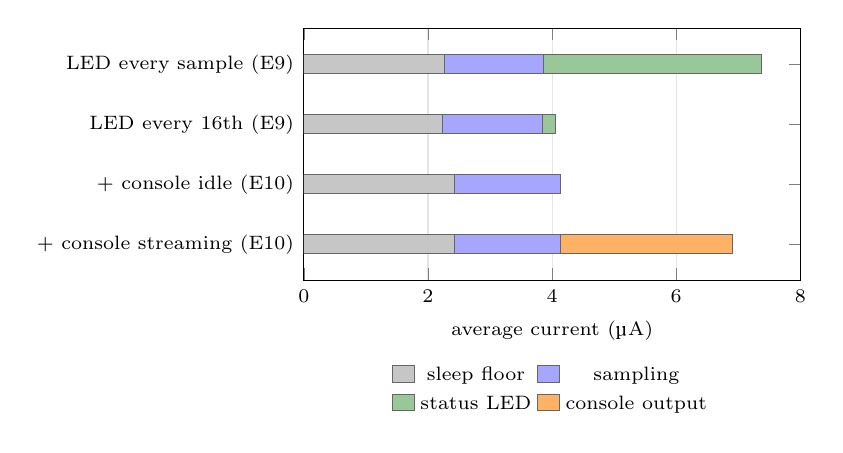
\begin{tikzpicture}
\begin{axis}[xbar stacked, scale only axis, width=0.52\columnwidth, height=3.2cm, bar width=7pt,
  xmin=0, xmax=8, xlabel={average current (\textmu A)},
  ymin=0.4, ymax=4.6, ytick={1,2,3,4},
  yticklabels={{+ console streaming (E10)},{+ console idle (E10)},{LED every 16th (E9)},{LED every sample (E9)}},
  tick label style={font=\scriptsize}, label style={font=\scriptsize},
  legend style={font=\scriptsize, at={(0.5,-0.3)}, anchor=north, legend columns=2, draw=none},
  xmajorgrids, grid style={gray!20}]
% y: 4 = LED every sample, 3 = LED every 16th, 2 = console idle, 1 = console streaming
\addplot[fill=gray!45, draw=black!60] coordinates {(2.26,4) (2.24,3) (2.42,2) (2.43,1)};
\addplot[fill=blue!35, draw=black!60] coordinates {(1.60,4) (1.60,3) (1.71,2) (1.71,1)};
\addplot[fill=green!45!black!40, draw=black!60] coordinates {(3.52,4) (0.22,3) (0,2) (0,1)};
\addplot[fill=orange!60, draw=black!60] coordinates {(0,4) (0,3) (0,2) (2.77,1)};
\legend{sleep floor, sampling, status LED, console output}
\end{axis}
\end{tikzpicture}
\caption{Average-current budget of the logger from two single-capture experiments. Each pair of bars shares one EnergyTrace session; floors differ by $\sim$0.2\uA{} between the sessions. The E10 build has no status LED.}
\label{fig:budget}
\end{figure}

Table~\ref{tab:energy} collects the measured averages and the resulting running time from a full supercapacitor. The usable charge is $C\,\Delta V = 0.22\times(3.3-2.2) = 0.242$\,C for logging, and $0.22\times(2.2-1.9) = 0.066$\,C for the deep-sleep hold that follows, down to about 1.9\,V, within the 1.8--1.99\,V range at which the high-side supply supervisor resets the device~\cite{ti_slase54}.

\begin{table}[t]
\caption{Measured average current and supercapacitor running time (leakage ignored)}
\label{tab:energy}
\centering\footnotesize
\begin{tabularx}{\columnwidth}{@{}Lrr@{}}
\toprule
Firmware (experiment) & Average & Running time \\
\midrule
Layer 1 demo, LED 25\,\% on (E2) & 780\uA & 5\,min \\
Logger, LED every sample (E6) & 7.86\uA & 8.6\,h \\
Final logger, LED every 16th, idle console (E8--E10) & 3.2--4.4\uA & 15--21\,h \\
Deep-sleep hold below 2.2\,V (E7) & $\sim$2.2\uA & +8\,h \\
\midrule
Final logger on the supercapacitor, from $C\,dV/dt$, leakage included (E11) & 5.4\uA & 8.5\,h$^{*}$ \\
\bottomrule
\multicolumn{3}{@{}l}{\scriptsize $^{*}$From 2.96 to 2.2\,V, the charge level reached in E11.}
\end{tabularx}
\end{table}

The final firmware's range reflects the measurement offset discussed next. E8 measured 3.21\uA{}. In the E9 and E10 sessions the same components add up to 4.1--4.4\uA, because their floors were higher.

\subsection{Running from the supercapacitor}

In E11 the final firmware ran from the supercapacitor alone, with USB unplugged, for 82\,min. Fig.~\ref{fig:drain} shows its history log, read back over the console after USB was reconnected. Over the first 10\,min the voltage fell at 47\,\textmu V/s. That is faster than the load explains and matches the charge redistribution expected in a freshly charged supercapacitor. From 30\,min on, the slope settled at 25.7\,\textmu V/s, and at 24.6\,\textmu V/s over the last 40\,min, with residuals within 2.6\,mV of a straight line. With $I = C\,dV/dt$, that is a total drain of 5.4--5.6\uA. The figure includes the capacitor's own leakage and everything on the supercapacitor side of the board, so it is the number that sets the real running time. It is 1--2\uA{} above the EnergyTrace measurements of the logger itself. At this rate the logger reaches the 2.2\,V cut-off 6.6--6.9\,h after the end of the run, or about 8.5\,h after the 2.96\,V the charge had reached. That is well short of the 15--21\,h estimated from EnergyTrace with leakage ignored.

The die temperature fell by 2\,\textdegree C in the first 10\,min after USB was unplugged and then stayed flat. That is consistent with self-heating from the board's USB debugger circuitry, which was powered during all the earlier readings.

The run also exercised the history and the clock recovery on hardware. Every power-on and reset-pin boot was logged, and the clock restarted after each one from the newest logged time, flagged as restored. The reset pin causes a brown-out-level reset on this device, so it clears the RTC as a power loss does. The sequence numbers and timestamps stayed in order across all of these boots.

\begin{figure}[t]
\centering
\begin{tikzpicture}
\begin{groupplot}[group style={group size=1 by 2, vertical sep=3mm, x descriptions at=edge bottom},
  width=\columnwidth, xmin=0, xmax=82, enlarge x limits=false,
  tick label style={font=\scriptsize}, label style={font=\scriptsize},
  grid=major, grid style={gray!20}, xlabel={time on the supercapacitor (min)}]
\nextgroupplot[height=4.2cm, ylabel={VCC (mV)}, ymin=2790, ymax=2975]
  \addplot[only marks, mark=*, mark size=1pt, blue!70!black] table[x=tmin, y=vcc] {data/e11_drain.dat};
  \addplot[red!70!black, dashed, domain=30:82] {2808 + 24.6e-3*60*(82.0-x)};
\nextgroupplot[height=2.6cm, ylabel={temp. (\textdegree C)}, ymin=26.8, ymax=29.6, ytick={27,28,29}]
  \addplot[only marks, mark=*, mark size=1pt, orange!80!black] table[x=tmin, y=temp] {data/e11_drain.dat};
\end{groupplot}
\end{tikzpicture}
\caption{Supercapacitor run (E11), one history record every 2\,min. The dashed line is the 24.6\,\textmu V/s fit over the last 40\,min, a 5.4\uA{} drain at 0.22\,F.}
\label{fig:drain}
\end{figure}

% =====================================================================
\section{Discussion}
\label{sec:discussion}

\subsection{Measurement pitfalls}

\emph{Debugger in control.} The first capture of the logger showed a constant 170\uA{} floor. That matches the datasheet's LPM0/LPM1 current with an 8\,MHz DCO (130--175\uA)~\cite{ti_slase54}, not LPM3. A code review found no firmware cause, and the same firmware captured in Free Run slept at 2.6\uA. A debug session in control of the device evidently kept the clock running.

\emph{Session-to-session offset.} With no firmware change in the sleep path, two captures showed floors of 2.62\uA{} and 1.35\uA. A test that switched firmware behaviour inside one capture (E9) gave the same floor in both halves, 2.256 and 2.243\uA. The same optimized firmware therefore read 1.35\uA{} in one session and 2.24\uA{} in another. The absolute microamp floor therefore varies by about 1\uA{} from one EnergyTrace session to the next. Event charges, such as the 7\uC{} LED flash, were consistent across sessions. Variants are therefore compared within one capture, and absolute floors are quoted as ranges.

\subsection{Limitations}

The EnergyTrace runtime estimates ignore the supercapacitor's own leakage. E11 shows that the leakage and the rest of the supercapacitor side of the board add 1--2\uA{} while logging, and they will matter more during the microamp-level deep-sleep hold. The measured LPM3.5 floor (2.1--2.25\uA) is well above the chip's datasheet value of about 0.5\uA~\cite{ti_slase54}. The remainder is attributed to the board and the measurement offset, but EnergyTrace cannot resolve it. After a real power loss the clock is restored from the last logged time, so it runs behind by the outage until it is set again. The supercapacitor run (E11) lasted 82\,min and covered only the top 150\,mV of the discharge, so the running time is an extrapolation. The full end-to-end scenario has not yet been run: discharging the supercapacitor through logging, cut-off and the deep-sleep hold, then reading the log back.

% =====================================================================
\section{Conclusions and Future Work}
\label{sec:conclusion}

A complete, register-level firmware stack for a supercapacitor-powered MSP430FR5994 logger was built and validated. State survives power loss by construction, which random power cuts and deterministic fault injection at every step of a save confirm. The device drops into LPM3.5 when energy runs low and resumes when it recovers, with continuous timekeeping. Measured with care, the logger draws 3.2--4.4\uA, about 200 times less than the first driver demo, and its console costs nothing while idle. On the supercapacitor itself the total drain is 5.4\uA, enough for about 8.5\,h of logging per charge. The measurement work showed that energy figures in the microamp range need debugger-free captures and same-capture comparisons to be trustworthy.

Future work:
\begin{itemize}
  \item extend E11 to the full supercapacitor discharge, from charged through the 2.2\,V cut-off and the LPM3.5 hold, and read the log over the console;
  \item measure the absolute sleep floor with an independent microammeter, and look for the board-level baseline, e.g.\ by removing the UART jumpers;
  \item add energy harvesting (for example a small solar cell) and adapt the sampling rate to the stored energy, in the direction of~\cite{colin2018capybara,hester2017future};
  \item measure the supercapacitor's leakage on its own, to separate it from the board's share of the 1--2\uA{} gap;
  \item firmware enhancements found in testing and in an interrupt-handling review:
  \begin{itemize}
    \item enter deep sleep only after two consecutive readings below 2.2\,V. A single reading taken during a supply dip, when J8 was moved and USB reconnected, sent the logger into LPM3.5. A real discharge through 2.2\,V takes hours, so the extra 2\,s cost nothing;
    \item close a lost-wake-up race in the timer's sleep helper. It tests its done flag with interrupts enabled before entering LPM3. If the timer fires in between, the CPU sleeps until the next interrupt, normally the 2\,s RTC tick, so a 2\,ms LED flash can last up to 2\,s. The fix is the disable--check--sleep sequence the main loop already uses;
    \item make the timer driver's read-modify-write updates of its status bytes atomic with critical sections, since its interrupt handler changes other bits of the same bytes;
    \item keep sampling during long console commands. Sample requests coalesce while a command runs, so a full \code{hist} dump ($\sim$1.5\,min) skips about 45 samples;
    \item restore the caller's interrupt state in the UART's blocking write and flush, which currently always return with interrupts enabled.
  \end{itemize}
\end{itemize}

\section*{Acknowledgment and AI Disclosure}
This work was prepared with the assistance of Claude (Anthropic), an AI assistant. Under the author's direction, it wrote the firmware, analysed the EnergyTrace data, drafted the text and figures, and checked the references against online bibliographic records (publisher, DOI and repository pages) and the cited Texas Instruments documents. The author ran all hardware experiments and is responsible for the content.

\bibliographystyle{IEEEtran}
\bibliography{references}

% =====================================================================
\onecolumn
\appendices

\section{Implementation Details}

\begin{table}[H]
\centering\small
\caption{Layer 1 drivers}
\begin{tabularx}{\textwidth}{@{}llL@{}}
\toprule
Driver & Responsibility & Key details \\
\midrule
hal\_common & Critical sections & \code{hal\_enter\_critical} / \code{hal\_exit\_critical} save and restore GIE \\
gpio & Ports P1--P8, PJ & Register-pointer table; PxSELC for 01$\leftrightarrow$10 function changes; driver owns PORT1--8 ISRs, loops on PxIV, callbacks return ``wake main'' \\
board & LaunchPad bring-up & Hold WDT $\rightarrow$ capture reset cause $\rightarrow$ all pins low $\rightarrow$ LEDs, buttons, UART idle, crystal pins $\rightarrow$ before-unlock hook $\rightarrow$ clear LOCKLPM5 $\rightarrow$ clear IFGs only if not an LPMx.5 wake; \code{board\_uart\_pins()} for the backchannel \\
cs & Clocks & DCO 1--16\,MHz with CS12 workaround and FRAM wait states (NWAITS\_1 above 8\,MHz); LFXT start with timeout, fallback to VLO; ms/\textmu s delays \\
pmm & Power and resets & Reset-cause bitmask from SYSRSTIV; boot reason; LPM0--4 entry from RAM; LPMx.5 entry; software BOR/POR \\
wdt & Watchdog & Watchdog and interval modes, kick, pause/resume; driver owns WDT\_VECTOR \\
\bottomrule
\end{tabularx}
\end{table}

\begin{table}[H]
\centering\small
\caption{Layer 2 and Layer 3 modules}
\begin{tabularx}{\textwidth}{@{}llL@{}}
\toprule
Module & Responsibility & Key details \\
\midrule
ref & Internal reference & 1.2 / 2.0 / 2.5\,V; waits on GENBUSY, polls REFGENRDY; TLV calibration factors with sanity check \\
adc & VCC and die temperature & VCC via A31 (BATMAP) on the 2.0\,V reference, falling back to 1.2\,V below 2.4\,V; temperature via A30 (TCMAP) on 1.2\,V with TLV two-point calibration, averaged over 8 conversions; \SI{40}{\micro\second} sample time; ADC and REF off after each read \\
rtc & Calendar clock & Binary calendar mode; keeps time across LPM3.5; 125\,ms--2\,s periodic interrupt, minute/hour events, daily alarm; never clears interrupt flags during setup; \code{rtc\_to\_epoch}/\code{rtc\_from\_epoch} \\
timer & Timer\_A0--A4 on ACLK & Periodic, one-shot and sleep (LPM3) helpers; divider chosen automatically; up to 130\,s \\
crc & CRC16 hardware & CRC-16/CCITT-FALSE; self-test against a software reference (check value 0x29B1) \\
ckpt & Power-loss-safe store & Two FRAM slots (\code{\#pragma PERSISTENT}), 256-byte payload, commit order of Section~\ref{sec:design}; newest valid slot restored \\
uart & eUSCI\_A0--A3, 8N1 & TX ring buffer fed by the TX interrupt; RX callback in interrupt context; baud registers from the user's-guide procedure; refuses $N<3$ \\
console & Command line & Echo, backspace, Ctrl-C; line parsed in the main loop into up to 6 words; input arriving while a line waits is refused with a bell; printing without \code{printf} \\
history & Long FRAM log & 1600 $\times$ 14-byte records; invalidate, fill, commit mark; 16-bit sequence; persistent hint repaired at boot; unit-tested on a PC against torn records, a lagging or corrupt hint, ring and sequence wrap, and clearing \\
\bottomrule
\end{tabularx}
\end{table}

\noindent The linker stack is 512 bytes (RAM use 1.4 of 4\,KB). Red LED flashes at boot give the restart reason (1 power-on, 2 LPMx.5 wake, 3 reset pin, 4 watchdog, 5 software, 6 fault); button S1 shows a supply gauge and S2 erases the state.

\section{Experiment Record}

All experiments were run on 21 November 2026 on one MSP-EXP430FR5994. E1--E10 were powered over USB, with J8 removed for energy captures. E11 ran from the supercapacitor alone.

\begin{table}[H]
\centering\small
\caption{Summary of experiments}
\begin{tabularx}{\textwidth}{@{}llLl@{}}
\toprule
\# & Experiment & Result & Verdict \\
\midrule
E1 & Build verification & All configurations compile without warnings at -Ooff and -O2 & Pass \\
E2 & Layer 1 EnergyTrace profile & 780\uA{} average, LED = 95\,\% of energy, sleep 2.4\uA & Baseline \\
E3 & Abrupt power cuts & 36 cuts: 0 restore failures, 0 torn copies, 0 saves lost & Pass \\
E4 & Fault injection & 9/9 steps as predicted & Pass \\
E5 & LPM3.5 deep sleep on USB & 9/9 check-ins clean, exact 60\,s spacing & Pass \\
E6 & Logger EnergyTrace & 7.86\uA{} average, 2.62\uA{} floor (Free Run) & Pass \\
E7 & LPM3.5 EnergyTrace & 2.10--2.25\uA{} floor, $\sim$1\uC{} per check-in without test LEDs & Pass \\
E8 & Optimized logger EnergyTrace & 3.21\uA{} average, 1.35\uA{} floor & Pass \\
E9 & LED A/B test, one capture & 7.41 $\rightarrow$ 4.10\uA; floor 2.256 vs 2.243\uA & Pass \\
E10 & Console energy, one capture & Idle: no measurable cost; streaming: +5.5\uC{} per line & Pass \\
E11 & Supercapacitor run, 82\,min & 2961 $\rightarrow$ 2808\,mV; 5.4\uA{} total drain; history and clock recovery correct across 9 boots & Pass \\
\bottomrule
\end{tabularx}
\end{table}

\subsection*{E1. Build verification}
Every driver and every test mode (\code{CKPT\_STRESS\_TEST}, \code{CKPT\_FAULT\_TEST}, \code{LPM35\_TEST}, \code{LED\_AB\_TEST}, \code{CONSOLE\_E10\_TEST}) was compiled with the project's flags (\code{-vmspx -{}-data\_model=restricted -{}-use\_hw\_mpy=F5}, MPU enabled, TI MSP430 CGT 21.6.1) at -Ooff and -O2 without warnings. Enabling two test modes at once is rejected at compile time.

\subsection*{E2. Layer 1 energy profile}
The Layer 1 demo lit LED1 for 25\,\% of each $\sim$1\,s period and slept in LPM3 in between. Average 776--780\uA; LED on 3.11\mA; the LED took 95\,\% of the energy plus 4.6\,\% in transition bins; sleep floor $\approx$\,2.4\uA. This capture was taken with the debugger attached, before the Free Run practice was adopted.

\subsection*{E3. Abrupt power cuts}
With \code{CKPT\_STRESS\_TEST = 1} the firmware saves checkpoints continuously; each field derives from one counter, so a mixed copy is detectable. Each boot checks the restored copy and records the result in persistent FRAM.

\begin{table}[H]
\centering\small
\begin{tabular}{@{}lccccc@{}}
\toprule
Run & Cuts & restore\_fail & content\_bad & saves\_lost\_max & last\_saved vs samples \\
\midrule
1 & 10 & 0 & 0 & 0 & 110464 vs 110465 \\
2 & 26 & 0 & 0 & 0 & 264023 vs 264024 \\
\bottomrule
\end{tabular}
\end{table}
\noindent \code{last\_saved} is one behind the RAM counter because the halt landed inside an unfinished save; restore correctly returned the previous complete copy.

\subsection*{E4. Fault injection}
With \code{CKPT\_FAULT\_TEST = 1}, \code{ckpt\_save()} has six cut points that trigger a software brown-out reset at an exact step; steps 7--9 corrupt FRAM directly.

\begin{table}[H]
\centering\small
\begin{tabularx}{\textwidth}{@{}lLl@{}}
\toprule
Step & Fault & Required outcome \\
\midrule
1 & Reset after the slot is marked invalid & Old copy restored \\
2 & Reset with half the payload written & Old copy restored \\
3 & Reset after the payload, before length and sequence & Old copy restored \\
4 & Reset after length and sequence, before the CRC & Old copy restored \\
5 & Reset after the CRC, before the commit & Old copy restored \\
6 & Reset just after the commit & New copy restored \\
7 & One payload bit flipped in the newest slot & Falls back to the older copy \\
8 & One header bit flipped in the remaining slot & Restore reports failure \\
9 & Save after both copies are lost & New copy restored \\
\bottomrule
\end{tabularx}
\end{table}
\noindent Result: \code{passed} = 0x03FE (steps 1--9), \code{failed} = 0, \code{restarts} = 0, final counter 5, exactly as predicted (2 $\rightarrow$ 3 at step 6 $\rightarrow$ 4 saved then corrupted $\rightarrow$ 5).

\subsection*{E5. LPM3.5 deep sleep on USB}
With \code{LPM35\_TEST = 1}, after 5 samples the low threshold is forced above VCC; the first two minute wakes stay asleep and the third applies the real 2.6\,V check. Each wake records its RTC time, gap, reset code and a fault mask in FRAM.

\begin{table}[H]
\centering\small
\begin{tabular}{@{}ccccc@{}}
\toprule
Episode & Asleep at (s) & Wakes (s) & First gap (s) & Resumed at (s) \\
\midrule
1 & 3 & 60, 120, 180 & 57 & 180 \\
2 & 187 & 240, 300, 360 & 53 & 360 \\
3 & 367 & 420, 480, 540 & 53 & 540 \\
\bottomrule
\end{tabular}
\end{table}
\noindent All nine wakes had reset code 8 (LPMx.5 wake) and fault mask 0. An earlier run disturbed by a reflash and a replug showed three timing faults; the clean rerun attributes them to that disturbance.

\subsection*{E6. Logger energy profile}
A first 300\,s capture under a debug session showed 175\uA{} average and a 170\uA{} floor; in Free Run the same firmware averaged 7.86\uA{} over complete sample periods, with a 2.62\uA{} floor and $\sim$10.4\uC{} per sample including the 2\,ms LED flash.

\subsection*{E7. LPM3.5 energy profile}
\code{LPM35\_TEST} build, 300\,s in Free Run, covering three hold wakes and two resumes. Floor 2.10--2.25\uA{} across six sleep stretches. A hold wake cost $\sim$640\uC{}, of which $\sim$638\uC{} were the test build's two 100\,ms LED flashes; the wake itself is estimated at $\sim$1\uC, about 0.02\uA{} averaged over a minute.

\subsection*{E8. Optimized logger}
Status LED only on log slot 0 (every 16th sample) and 8-conversion temperature averaging; 300\,s Free Run. Average 3.21\uA{} over complete sample periods, floor 1.35\uA. The floor's difference from E6 (2.62\uA) is constant over the whole sleep period; E9 shows it is a measurement-session offset.

\subsection*{E9. LED A/B test in one capture}
\code{LED\_AB\_TEST = 1} flashes the LED on every sample for the first 75 samples, then on every 16th.

\begin{table}[H]
\centering\small
\begin{tabular}{@{}lcccc@{}}
\toprule
Mode (same capture) & Periods & Floor & Average & Charge above floor \\
\midrule
LED every sample & 71 & 2.256\uA & 7.41\uA & 10.25\uC{} \\
LED every 16th, all periods & 74 & 2.243\uA & 4.10\uA & -- \\
\quad samples without LED & 69 & 2.243\uA & 3.86\uA & 3.21\uC{} \\
\quad samples with LED & 5 & 2.248\uA & 7.41\uA & 10.21\uC{} \\
\bottomrule
\end{tabular}
\end{table}
\noindent The floor does not move at the switch (0.013\uA), so the firmware does not cause the E6/E8 difference. The LED flash costs 7.0\uC{} and the saving is 3.3\uA{} (45\,\%).

\subsection*{E10. Console energy cost}
\code{CONSOLE\_E10\_TEST = 1} runs three phases counted in samples from boot, with the status LED disabled: console off (samples 1--50), console on and idle (51--100, banner printed once), console streaming one $\sim$36-character CSV line per sample (101 on). The first five samples after boot are excluded. A first attempt captured the normal build by mistake and was discarded.

\begin{table}[H]
\centering\small
\begin{tabular}{@{}lcccc@{}}
\toprule
Phase (same capture) & Periods & Floor & Average & Charge above floor \\
\midrule
Console off & 45 & 2.420\uA & 4.12\uA & 3.39\uC \\
Console on, idle & 48 & 2.421\uA & 4.13\uA & 3.40\uC \\
Console streaming & 49 & 2.428\uA & 6.90\uA & 8.90\uC \\
\bottomrule
\end{tabular}
\end{table}
\noindent Streaming costs about 0.15\uC{} per character. The boot banner costs $\sim$6.6\uC{} once.

\subsection*{E11. Supercapacitor run}
Normal build (all test switches 0). On USB, the history was cleared and the board was reset, power-cycled and reset again to exercise the boot records (records 1--9). The clock was set (record 10, the date left at 2026-01-01). J8 was then moved to Use and USB was unplugged; the move caused a power-on reset at 2954\,mV (record 11). The board logged on the supercapacitor for 82\,min (records 12--53) until USB was reconnected (record 54, power-on at 3296\,mV). The \code{hist} dump is kept in \code{report/data/e11\_hist.csv}.

\begin{table}[H]
\centering\small
\begin{tabular}{@{}lccc@{}}
\toprule
Window & Records & Slope & Current at 0.22\,F \\
\midrule
First 10\,min & 6 & 46.7\,\textmu V/s & (10.3\uA, charge redistribution) \\
From 30\,min & 27 & 25.7\,\textmu V/s & 5.64\uA \\
Last 40\,min & 21 & 24.6\,\textmu V/s & 5.41\uA \\
\bottomrule
\end{tabular}
\end{table}
\noindent All boots after the first two were flagged ``clock restored'', including the three reset-pin boots: the RST pin is a brown-out-level reset and clears the RTC. After the final reconnect the clock restarted at 73078\,s, one second after the newest entry in the checkpoint's sample log, which ran 2\,min past the last history record. The temperature fell from 29.2 to 27.2\,\textdegree C in the first 10\,min unplugged.

\section{Files and Build Switches}

\begin{table}[H]
\centering\small
\begin{tabularx}{\textwidth}{@{}lL@{}}
\toprule
Path & Contents \\
\midrule
\code{drivers/msp430/} & hal\_common, gpio, cs, pmm, wdt, ref, adc, rtc, timer, crc, ckpt, uart \\
\code{drivers/board/} & LaunchPad bring-up and pin map (board) \\
\code{app/console.*} & Command console \\
\code{main.c} & Logger, console commands and the test modes \\
\code{report/} & This paper (\code{lab\_report.tex}), \code{references.bib}, plot data in \code{data/} \\
\code{dvt/*.csv} & EnergyTrace captures of E2 and E6--E10 \\
\bottomrule
\end{tabularx}
\end{table}

\begin{table}[H]
\centering\small
\begin{tabularx}{\textwidth}{@{}llL@{}}
\toprule
Switch & File & Effect when 1 \\
\midrule
\code{CKPT\_STRESS\_TEST} & \code{main.c} & Continuous saves for unplug testing (E3) \\
\code{CKPT\_FAULT\_TEST} & \code{drivers/msp430/ckpt.h} & Cut points in \code{ckpt\_save}, fault sequence (E4) \\
\code{LPM35\_TEST} & \code{main.c} & Scheduled LPM3.5 episodes on USB (E5, E7) \\
\code{LED\_AB\_TEST} & \code{main.c} & LED every sample for 75 samples, then every 16th (E9) \\
\code{CONSOLE\_E10\_TEST} & \code{main.c} & Console off / idle / streaming in one capture (E10) \\
\code{ADC\_TEMP\_AVG} & \code{drivers/msp430/adc.h} & Conversions averaged per temperature reading (default 8) \\
\bottomrule
\end{tabularx}
\end{table}

\noindent Only one test switch may be 1 at a time. Test results in FRAM are re-initialised by a program download and can be read without reflashing by connecting the debugger and loading symbols only.

\end{document}
